\documentclass[tikz]{standalone}
\usepackage{pgfplots}
\pgfplotsset{compat=1.18}
\begin{document}
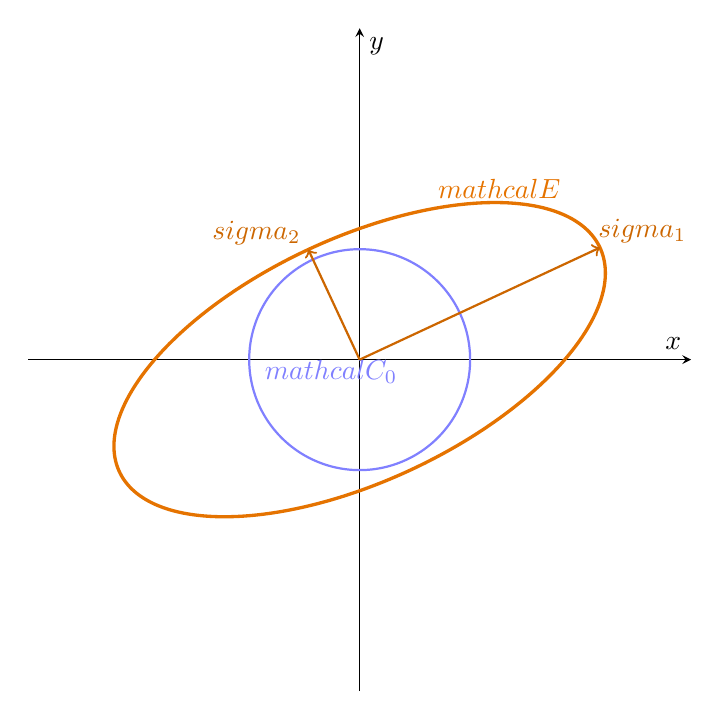
\begin{tikzpicture}
  \begin{axis}[
      axis lines=middle,
      xmin=-3, xmax=3,
      ymin=-3, ymax=3,
      xlabel={$x$}, ylabel={$y$},
      ticks=none,
      width=10cm, height=10cm,
      clip=false
  ]
    \pgfmathsetmacro{\sigmaOne}{2.4}
    \pgfmathsetmacro{\sigmaTwo}{1.1}
    \pgfmathsetmacro{\theta}{25}
    \pgfmathsetmacro{\sigOneX}{\sigmaOne*cos(\theta)}
    \pgfmathsetmacro{\sigOneY}{\sigmaOne*sin(\theta)}
    \pgfmathsetmacro{\sigTwoX}{-\sigmaTwo*sin(\theta)}
    \pgfmathsetmacro{\sigTwoY}{\sigmaTwo*cos(\theta)}

    \addplot[blue!50, thick, samples=200, domain=0:360]
      ({cos(x)}, {sin(x)}) node[pos=0.55, above right] {$\\mathcal{C}_0$};

    \addplot[orange!90!black, very thick, samples=300, domain=0:360]
      ({\sigmaOne*cos(\theta)*cos(x) - \sigmaTwo*sin(\theta)*sin(x)},
       {\sigmaOne*sin(\theta)*cos(x) + \sigmaTwo*cos(\theta)*sin(x)})
      node[pos=0.15, above right] {$\\mathcal{E}$};

    \draw[->, thick, orange!80!black] (axis cs:0,0) -- (axis cs:\sigOneX,\sigOneY) node[pos=0.95, above right] {$\\sigma_1$};
    \draw[->, thick, orange!80!black] (axis cs:0,0) -- (axis cs:\sigTwoX,\sigTwoY) node[pos=0.95, above left] {$\\sigma_2$};
  \end{axis}
\end{tikzpicture}
\end{document}
